\begin{figure*}[t]
\centering
\begin{minipage}[t]{0.49\textwidth}
  \centering
  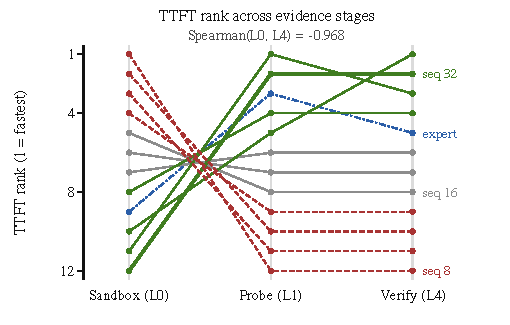
\includegraphics[width=\linewidth]{figures/results/fig6a_rank_inversion.pdf}
\end{minipage}\hfill
\begin{minipage}[t]{0.49\textwidth}
  \centering
  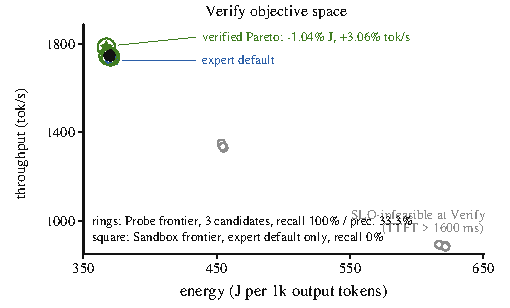
\includegraphics[width=\linewidth]{figures/results/fig6b_objective_space.pdf}
\end{minipage}
\caption{Why full verification remains necessary.  Left: Sandbox TTFT ranking
is nearly reversed relative to Verify ($\rho=-0.968$); the measured Probe
repairs most of the ordering.  Right: The zoomed objective space contains the
five SLO-feasible Verify candidates; seven infeasible candidates lie outside
the plotted window.  Rings denote the three-candidate Probe frontier, the
square denotes the Sandbox frontier, and the star marks the unique verified
Pareto configuration.  Probe avoids a false negative, while Verify removes its
two false positives.}
\label{fig:configuration-fidelity}
\end{figure*}
